\documentclass[UTF8, 12pt, a4paper, fleqn]{ctexart}
\usepackage{geometry}
\usepackage{amsmath}
\usepackage{arydshln}
\usepackage{graphicx}
\usepackage{listings}
\usepackage{xcolor}
\geometry{left=2.0cm, right=2.0cm, top=1.0cm, bottom=2.5cm}

\title{PRML-第二章作业}
\author{}
\date{}
\begin{document}
\pagestyle{plain}
    \maketitle
    \subsection*{1. 书面作业}
    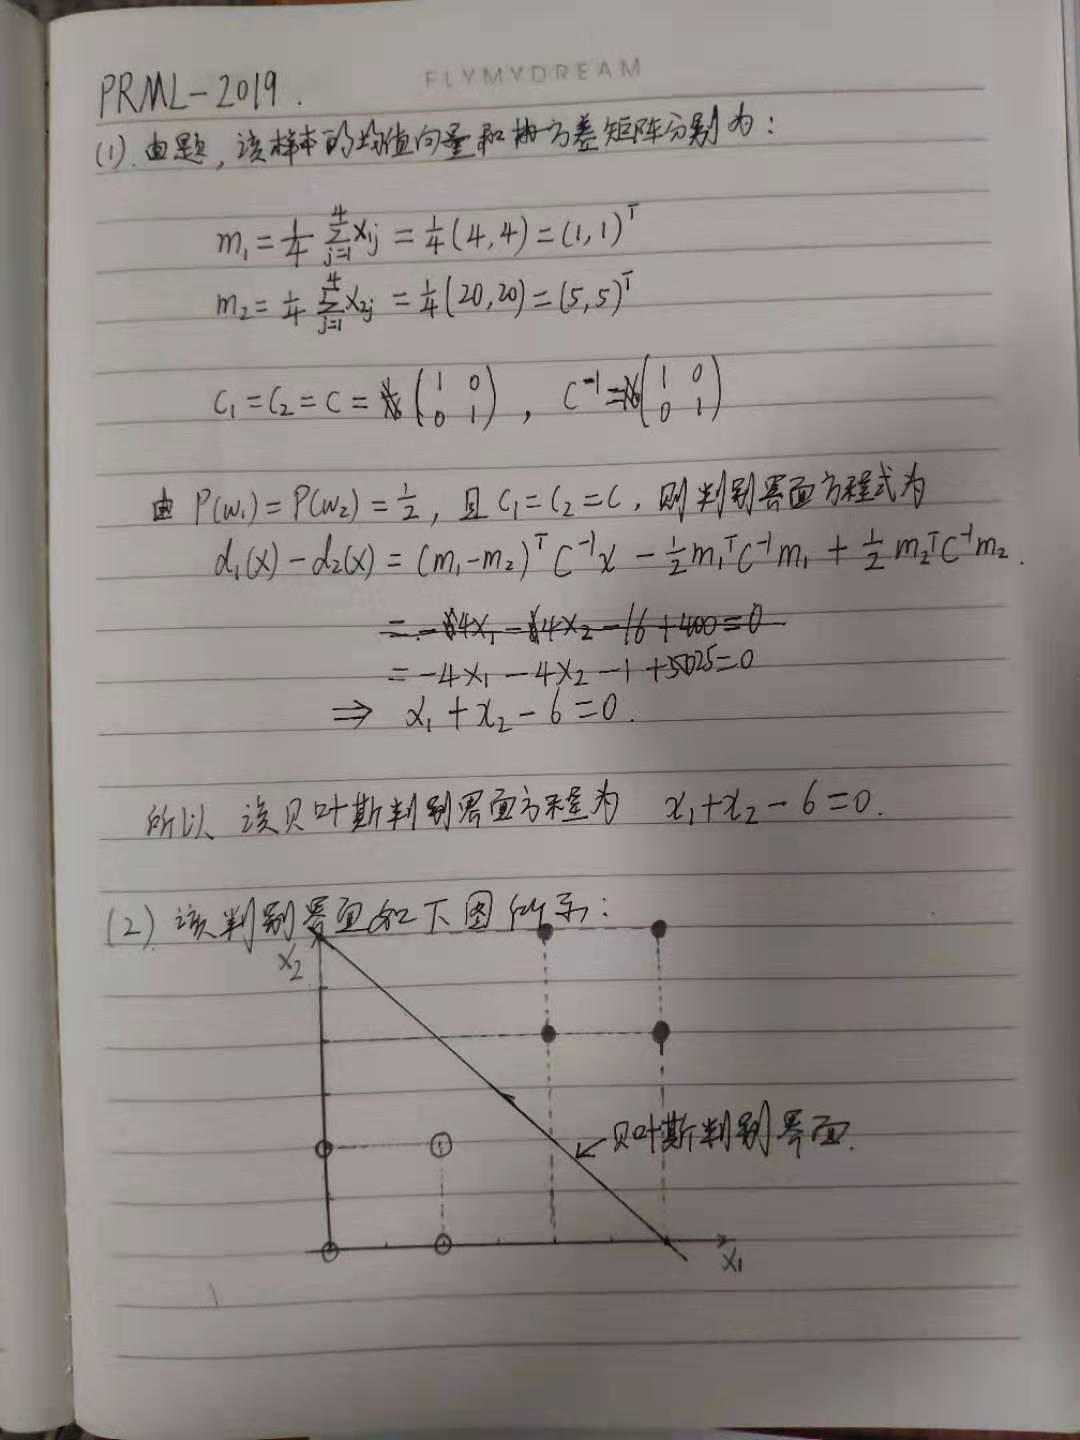
\includegraphics[scale=0.4]{assignment1.jpg}
    \subsection*{2. 编程作业}
    \lstset{
    %backgroundcolor=\color{red!50!green!50!blue!50},%代码块背景色为浅灰色
    rulesepcolor= \color{gray}, %代码块边框颜色
    breaklines=true,  %代码过长则换行
    % numbers=left, %行号在左侧显示
    % numberstyle= \small,%行号字体
    %keywordstyle= \color{blue},%关键字颜色
    commentstyle=\color{gray}, %注释颜色
    frame=shadowbox%用方框框住代码块
    }
     
    \begin{lstlisting}[language={Python}] 
import matplotlib.pyplot as plt
import numpy as np
import math

#坐标数据
a = np.array([[0.,2.,2.,0.], [0.,0.,2.,2.]], dtype=np.float64)
b = np.array([[4.,6.,6.,4.], [4.,4.,6.,6.]], dtype=np.float64)

#计算均值向量和协方差矩阵
a_t=np.matrix(a)
b_t = np.matrix(b)
m1 = np.matrix(a.mean(axis=1)).T
m2 = np.matrix(b.mean(axis=1)).T

c1 = np.cov(a_t) / 4 * 3
c2 = np.cov(b_t) / 4 * 3
c1_i = np.linalg.inv(c1)
c2_i = np.linalg.inv(c2)
c_i =c1_i

d1 = np.matmul((m1-m2).T, c_i)
k1 = 1/2 * np.matmul(np.matmul(m1.T, c_i),m1) - 1/2 * np.matmul(np.matmul(m2.T, c_i), m2)

#根据公式得到x2关于x1的直线作为分类的分界线
x = np.arange(0,7,1)
y = k1[0,0]/d1[0,1] - (d1[0,0]*x)/d1[0,1]
# print(m1,'\n\n', c1, '\n\n', c1_i)
# print(m1,'\n\n', c2, '\n\n', c2_i)
# print(d1,d1[0,0], '\n\n', k1[0,0])
#画图
plt.plot(a[0],a[1],"ro")
plt.plot(b[0], b[1], "bo")
plt.plot(x,y)
plt.show()
    \end{lstlisting}
    改代码的运行结果如下图所示:\\
    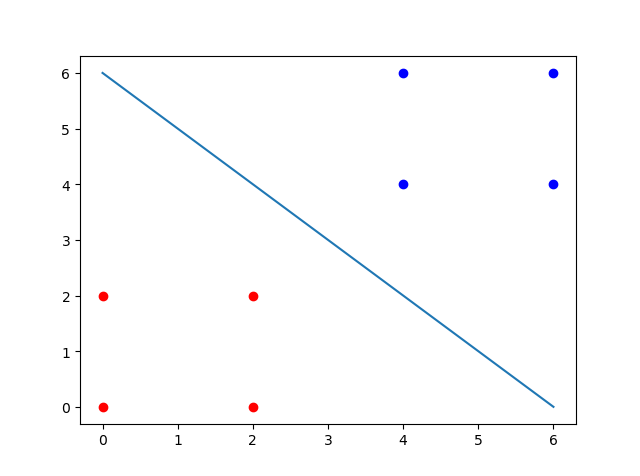
\includegraphics[]{Figure_1.png}



\end{document}